\documentclass[12pt,a4paper,notitlepage]{article}

\usepackage[utf8]{inputenc}

\usepackage[francais]{babel}\usepackage[T1]{fontenc}
\usepackage[cyr]{aeguill}
\usepackage{lmodern}
\usepackage{color}
\usepackage{boites}
\usepackage{caption}
\usepackage{fancybox}
\usepackage{listings}
%\lstset{language=bash, basicstyle=\footnotesize, frame=shadowbox, rulesepcolor=\color{gris}, captionpos=b}

  \lstset{
         basicstyle=\footnotesize\ttfamily, % Standardschrift
         %numbers=left,               % Ort der Zeilennummern
         numberstyle=\tiny,          % Stil der Zeilennummern
         %stepnumber=2,               % Abstand zwischen den Zeilennummern
         numbersep=5pt,              % Abstand der Nummern zum Text
         tabsize=2,                  % Groesse von Tabs
         extendedchars=true,         %
         breaklines=true,            % Zeilen werden Umgebrochen
         keywordstyle=\color{red},
                frame=b,         
         keywordstyle=[1]{\itshape}{//},    % Stil der Keywords
         stringstyle=\color{white}\ttfamily, % Farbe der String
         showspaces=false,           % Leerzeichen anzeigen ?
         showtabs=false,             % Tabs anzeigen ?
         xleftmargin=5pt,
         framexleftmargin=1pt,
         framexrightmargin=5pt,
         %numbers=left,
         frame=toplines,
         framextopmargin=3pt,
       %  framexleftmargin=8pt,
         numberblanklines=false,
         %morecomment=[s][marron]{/*}{*/},
         %moredelim=*[s][\color{blue}]{/*}{*/}
         %morecomment=[s][marron]{/*-}{*/}},         
         framexbottommargin=5pt,
         captionpos=b,
         %backgroundcolor=\color{lightgray},
         showstringspaces=false      % Leerzeichen in Strings anzeigen ? 
 }

\DeclareCaptionFont{white}{\color{white}}
\DeclareCaptionFormat{listing}{\colorbox[cmyk]{0.43, 0.35, 0.35,0.01}{\parbox{\textwidth}{\hspace{10pt}#1#2#3}}}
\captionsetup[lstlisting]{format=listing,labelfont=white,textfont=white, singlelinecheck=false, margin=0pt, font={bf,footnotesize}}

\definecolor{gris}{gray}{0.75}
%\definecolor{bleup}{HTML}{258EE9}


%\renewcommand*\familydefault{\ttdefault} %% Only if the base font of the document is to be typewriter style
%\renewcommand{\rmdefault}{ptm}


\usepackage[
   pdfauthor={Ludovic Terrier & Arnaud Goulut},
   pdftitle={RE12 - TP2},
   ]{hyperref}
   
   
\usepackage[pdftex]{graphicx}

%\usepackage{titlesec}
%\titleformat{\section}[frame] {\normalfont} {\filright
%\footnotesize
%\enspace\textbf{\thesection}\enspace} {8pt} {\Large\bfseries\filcenter}

%% Je contrôle la taille de ma zone imprimée...
\usepackage{anysize}
%% ...en définissants les marges {gauche}{droite}{haute}{basse}
\marginsize{25mm}{15mm}{10mm}{15mm}

\begin{document}

\title{La résolution des noms}
\author{Arnaud Goulut et Ludovic Terrier}
\date{Avril 2010}
\maketitle


%\tableofcontents

\thispagestyle{empty}


%%%%%%%%%%%%%%%%%%%%%%%%%%%%%%%%%%%  1ère page 


%%%%%%%%%%%%%%%%%%%%%%%%%%%%%%%%%%% 1ère partie
\section{Le DNS côté client}

\subsection{Le fichier \texttt{/etc/resolv.conf}}
Pour utiliser le serveur DNS de l'UTT (\texttt{193.50.230.240}) depuis le réseau de l'UTT, il faut écrire dans le fichier \texttt{/etc/resolv.conf} : \\

\begin{lstlisting}[title=Contenu du fichier resolv.conf]
nameserver 193.50.230.240
search utt.fr
\end{lstlisting}

\bigskip
On peut renseigner plusieurs paramètres dans ce fichier, en voici trois exemples :
\begin{itemize}
\item nameserver : l'adresse du DNS à utiliser pars la machine,
\item search : ajoute automatiquement ce suffixe lors des résolutions,
\item domain : définit le domaine auquel appartient la machine.
\end{itemize}


\subsection{L'outil dig}
La commande \texttt{dig} permet d'effectuer des requêtes DNS et d'en lire le résultat à l'écran. On peut l'utiliser pour effectuer différents types de requêtes que l'on va aborder dans cette partie.

\subsubsection{Directe}

Une requête directe sur un nom de domaine s'obtient avec la commande : \texttt{dig nomDeDomaine in A}, voyons à présent le résultat de la requête : \texttt{dig flickr.com in A}
\begin{lstlisting}[title=Résultat d'une requête directe]
;; QUESTION SECTION:
;flickr.com.                    IN      A

;; ANSWER SECTION:
flickr.com.             335     IN      A       68.142.214.24

;; AUTHORITY SECTION:
flickr.com.             76681   IN      NS      ns2.yahoo.com.
flickr.com.             76681   IN      NS      ns5.yahoo.com.
flickr.com.             76681   IN      NS      ns3.yahoo.com.
flickr.com.             76681   IN      NS      ns1.yahoo.com.

;; Query time: 60 msec
;; SERVER: 212.27.40.241#53(212.27.40.241)
;; WHEN: Sat May  1 14:43:58 2010
;; MSG SIZE  rcvd: 140
\end{lstlisting}

La réponse comporte quatre champs d'information :
\begin{itemize}
\item{Question section :} exprime sur une ligne un résumé de la requête effectuée,
\item{Answer section :} c'est la réponse, contenant l'adresse (ou les adresses) IP de la machine testée (ici le serveur web de flickr.com), ainsi que le TTL\footnote{Time To Live}, durée de validité de l'information en secondes,
\item{Authority section :} ce sont l'ensemble des serveurs DNS qui ont autorité sur la zone,
\item{Informations :} Durée de la requête, l'adresse IP du serveur qui a répondu, la date, et la taille du message reçu (en octets).
\end{itemize}

\subsubsection{Inverse}
 \texttt{dig} permet d'obtenir le nom de domaine associé à une adresse IP. Le résultat s'obtient avec la commande : \texttt{dig -x 193.50.230.240} ce qui est plus simple à utiliser que : 

\noindent \texttt{dig 240.230.50.193.in-addr.arpa. in PTR}\\
\begin{lstlisting}[title=Contenu d'une requête inverse]
;; QUESTION SECTION:
;240.230.50.193.in-addr.arpa.   IN      PTR

;; ANSWER SECTION:
240.230.50.193.in-addr.arpa. 86400 IN   PTR     pluton.utt.fr.

;; AUTHORITY SECTION:
230.50.193.in-addr.arpa. 86400  IN      NS      pluton.utt.fr.
230.50.193.in-addr.arpa. 86400  IN      NS      orion.utc.fr.

;; Query time: 68 msec
;; SERVER: 212.27.40.241#53(212.27.40.241)
;; WHEN: Sat May  1 14:52:08 2010
;; MSG SIZE  rcvd: 110
\end{lstlisting}

\subsubsection{Mail exchange}
On peut aussi tester l'adresse d'un serveur de mail via la requête mail exchange (MX), avec \texttt{dig} cela s'obtient avec la commande : \texttt{dig utbm.fr in MX}\\
\begin{lstlisting}[title=Contenu d'une requête de type Exchange Mail]
;; QUESTION SECTION:
;utbm.fr.                       IN      MX

;; ANSWER SECTION:
utbm.fr.                259200  IN      MX      1 serveur2314.utbm.fr.

;; AUTHORITY SECTION:
utbm.fr.                259200  IN      NS      pluton.utt.fr.
utbm.fr.                259200  IN      NS      portail1.utbm.fr.
utbm.fr.                259200  IN      NS      portail2.utbm.fr.
utbm.fr.                259200  IN      NS      portail5.utbm.fr.

;; ADDITIONAL SECTION:
serveur2314.utbm.fr.    259200  IN      A       193.48.231.4
portail1.utbm.fr.       600     IN      A       193.48.246.2
portail2.utbm.fr.       259200  IN      A       193.48.246.11
portail5.utbm.fr.       259200  IN      A       193.48.246.16

;; Query time: 84 msec
;; SERVER: 212.27.40.241#53(212.27.40.241)
;; WHEN: Sat May  1 15:03:15 2010
;; MSG SIZE  rcvd: 211
\end{lstlisting}


\clearpage
\subsection{L'outil whois}
La commande \texttt{whois} permet de récupérer l'ensemble des informations concernant un nom de domaine telles que le propriétaire, le nom de l'organisation qui le gère, le nom des personnes à joindre en cas de réclamation ou problème, accompagné de leur numéro de téléphone et la date d'expiration par exemple.
Ci-dessous un exemple avec le domaine \texttt{fedoraproject.org} :\\
\begin{lstlisting}[title=Résultat de la commande whois]
Domain ID:D101496757-LROR
Domain Name:FEDORAPROJECT.ORG
Created On:24-Sep-2003 10:32:11 UTC
Last Updated On:23-Jul-2009 17:52:39 UTC
Expiration Date:24-Sep-2010 10:32:11 UTC
Sponsoring Registrar:Network Solutions LLC (R63-LROR)
Status:CLIENT TRANSFER PROHIBITED
Registrant ID:41295926-NSI
Registrant Name:Red Hat, Inc.
Registrant Organization:Red Hat, Inc.
Registrant Street1:1801 Varsity Drive
Registrant City:Raleigh
Registrant State/Province:NC
Registrant Postal Code:27606
Registrant Country:US
Registrant Phone:+1.919754370
Registrant FAX:+1.919754370
Registrant Email:domainadmin@redhat.com
Admin ID:41295926-NSI
Admin Name:Red Hat, Inc.
Admin Organization:Red Hat, Inc.
Admin Street1:1801 Varsity Drive
Admin City:Raleigh
Admin State/Province:NC
Admin Postal Code:27606
Admin Country:US
Admin Phone:+1.919754370
Admin FAX:+1.919754370
Admin Email:domainadmin@redhat.com
Tech ID:41434783-NSI
Tech Name:Fedora Project
Tech Street1:Red Hat
Tech Street2:1801 Varsity Drive
Tech City:Raleigh
Tech State/Province:NC
Tech Postal Code:27606
Tech Country:US
Tech Phone:+1.919754370
Tech Email:admin@fedora.redhat.com
Name Server:NS1.FEDORAPROJECT.ORG
Name Server:NS2.FEDORAPROJECT.ORG
DNSSEC:Unsigned
\end{lstlisting}

\clearpage
\section{Mise en \oe uvre d'un serveur DNS relai}
%Le serveur
\subsection{Installation de Bind9}

L'installation du serveur Bind9 se fait, en root, via la commande : \texttt{yum install bind}
\begin{lstlisting}[title=Contenu du fichier named.conf]
options {
        listen-on port 53 { 192.168.3.129; };
        listen-on-v6 port 53 { ::1; };
        directory       "/var/named";
        dump-file       "/var/named/data/cache_dump.db";
        statistics-file "/var/named/data/named_stats.txt";
        memstatistics-file "/var/named/data/named_mem_stats.txt";
        allow-query     { localhost; 192.168.3.0/24; };
        recursion yes;
        forward first;
        forwarders {
        193.50.230.240 port 53;
        };
};

logging {
        channel default_debug {
                file "data/named.run";
                severity dynamic;
        };
};

zone "." IN {
        type hint;
        file "named.ca";
};

include "/etc/named.rfc1912.zones";
\end{lstlisting}

Après avoir installé le serveur \texttt{bind} il suffit d'éditer le fichier \texttt{/etc/named.conf} en y ajoutant la partie : 
\begin{center}
	\begin{verbatim}
	forwarders {
		193.50.230.240 port 53;
		};
	\end{verbatim}
\end{center}

Ceci signifie que toutes les requêtes DNS qui vont être faites à cette machine seront transférées au serveur DNS de l'UTT :  193.50.230.240.\\

Cependant pour que le serveur écoute l'interface connectée, on doit aussi ajouter :
\begin{verbatim}
listen-on	port	53	{	192.168.3.129;	};
\end{verbatim}



\subsection{Configuration du resolver}
Pour que le serveur que nous venons de configurer soit utilisé par les machines de notre réseau, il suffit de remplacer l'adresse IP de l'ancien DNS présent dans le fichier \texttt{/etc/resolv.conf} par celle du serveur faisant office de relai (ici 192.168.1.129). 

\subsection{Fonctionnement du relai}

\begin{figure}[!h]
\begin{center}
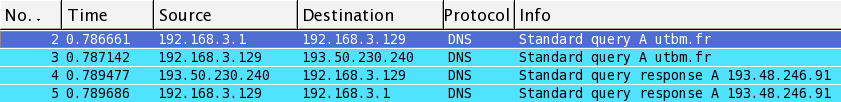
\includegraphics[scale=0.61]{capture-via-relai}
\caption{Requête DNS via un relai.}
\label{fig:da}
\end{center}
\end{figure}

Dans cette capture, on voit que le client effectue sa requête sur le serveur relai (\texttt{192.168.3.129}) et que ce dernier refait exactement la même à destination du serveur de l'UTT. Il reçoit ensuite la réponse, et la renvoie à l'identique au client. Le serveur fonctionne donc bien en mode relai, fonctionnalité qui est utile pour centraliser les requêtes et ainsi profiter du cache pour tous les utilisateurs. Mais cela permet également de connaître l'ensemble des demandes qui ont été réalisées.



\section{Résolution du domaine b3.re12.fr}

Nous allons à présent créer une zone b3.re12.fr gérée par notre machine faisant office de serveur DNS.

\subsection{Configuration}

Pour pouvoir gérer la zone b3.re12.fr il faut effectuer deux opérations :
\begin{itemize}
\item ajouter dans le fichier \texttt{/etc/named.conf} la gestion de cette zone,
\item créer le fichier contenant l'ensemble des paramètres de la zone.
\end{itemize}

\bigskip

\subsubsection{Modification du fichier \texttt{/etc/named.conf}}

\begin{lstlisting}[title=Lignes à ajouter]
zone "b3.re12.fr" IN {
        type master;
        file "db.b3.re12.fr";
};
\end{lstlisting}

Ici, on signifie au serveur que le fichier de configuration de la zone b3.re12.fr se nomme : db.b3.re12.fr. Voir le début du fichier \texttt{/etc/named.conf} qui indique que le serveur bind trouvera les configurations des zones dans le dossier \texttt{/var/named}

\subsubsection{Création du fichier \texttt{/var/named/db.b3.re12.fr}}

\begin{lstlisting}[title=Ensemble des paramètres de la zone]
$TTL 3h
@       IN      SOA     ns.b3.re12.fr. hostmaster.b3.re12.fr. (
                                2010051102
                                8H
                                2H
                                1W
                                1D )

@       IN      NS      ns.b3.re12.fr.

@       IN      MX   10   mail.b3.re12.fr.

pc-arnaud       IN A 192.168.3.1
pc-ludo         IN A 192.168.3.129
router-ludo     IN A 192.168.3.254
router-arnaud   IN A 192.168.3.126
ns              IN NS 192.168.3.129
mail            IN A 192.168.3.129
\end{lstlisting}

Ainsi, dans ce fichier on renseigne les paramètres de conservation de la réponse DNS,  le nom du serveur DNS de la zone (champ NS), le nom du serveur de mails (champ MX) et enfin la correspondance entre toutes les machines que l'ont souhaite gérer avec leur adresse IP. 

\clearpage
\subsection{La résolution inverse}

\subsubsection{Modification du fichier \texttt{/etc/named.conf}}

On ajoute ce bloc au fichier \texttt{/etc/named.conf} afin que le serveur prenne en compte la résolution inverse.

\begin{lstlisting}[title=Ajout de la zone inverse à gérer]
zone "3.168.192.in-addr.arpa" IN {
        type master;
        file "db.3.168.192.in-addr.arpa";
};
\end{lstlisting}

\subsubsection{Création du fichier \texttt{/var/named/db3.inv}}
De la même manière que pour la résolution directe, on créé un fichier contenant les informations relatives à la validité des réponses ainsi que la correspondance entre l'adresse IP et le nom des machines. (PTR désignant la requête inverse).
\begin{lstlisting}[title=Paramètres de la zone inverse]
$TTL    604800
@       IN      SOA     ns.b3.re12.fr. root.b3.re12.fr.     (
                2010042701 ; Serial (date + incrementation)
                7200       ; Refresh
                3600       ; Retry
                1209600    ; Expire
                604800     ; Negative Cache TTL
                )

A 192.168.3.1
A 192.168.3.129
A 192.168.3.254
A 192.168.3.126
NS 192.168.3.129
A 192.168.3.129

1                 PTR     pc-arnaud
129               PTR     pc-ludo
254               PTR     router-ludo
126               PTR     router-arnaud
\end{lstlisting}


\clearpage
\section{Mise en place d'un serveur secondaire}

Dans cette partie, nous avons configuré un second serveur afin qu'il agisse comme un DNS secondaire (\texttt{slave}). Au niveau de la configuration, il suffit d'indiquer dans le fichier \texttt{/etc/named.conf} que le contenu de la zone est à récupérer sur le serveur primaire (i.e. \texttt{master}).\\


\begin{lstlisting}[title=Configuration du serveur secondaire]
zone "b3.re12.fr" IN {
	type slave;
	masters {192.168.3.129;} ;
};
\end{lstlisting}\bigskip
On peut ensuite vérifier le bon fonctionnement avec Wireshark :

\begin{figure}[!h]
\begin{center}
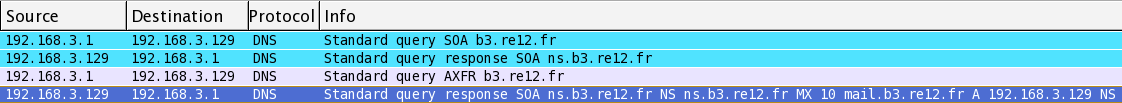
\includegraphics[scale=0.43]{dns-secondaire}
\caption{Requête de transfert de zone par le serveur secondaire.}
\label{fig:da}
\end{center}
\end{figure}

Dans cette capture, on voit que le serveur secondaire (\texttt{192.168.3.1}) effectue une requête de type \texttt{AXFR} pour récupérer les informations de la  zone b3.re12.fr.\\

En regardant plus précisément le contenu de la réponse donnée par le serveur maître (\texttt{192.168.3.129}) on voit l'ensemble des enregistrements de la zone b3.re12.fr.
\begin{figure}[!h]
\begin{center}
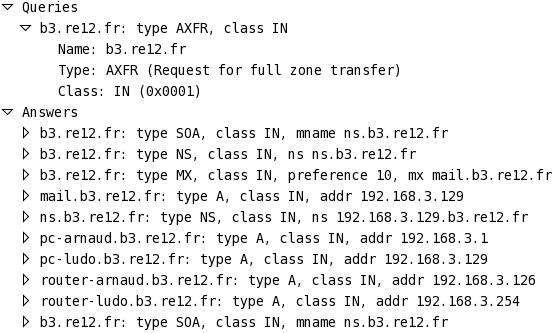
\includegraphics[scale=0.55]{axfr}
\caption{Question et réponse de la requête AXFR.}
\label{fig:da}
\end{center}
\end{figure}

\end{document}